% !TEX root = ../main_standard.tex
\chapter{Requirement and Analysis}
This chapter is to analysis the possible solutions according to the aims of the project as well as evaluation criteria. In section 3.1, the problem is divided into 3 parts which are modeling the spider, spider animation and spider rendering. Due to the time constraints, the project will mainly focus on spider animation. Initially a simple rendering for the spider is sufficient for the project. The Oculus Rift is also briefly introduced in this section 3.5. Section 3.6 and 3.7 are requirements lists and how the project will be evaluated. The final section is about ethics and legal considerations of the project.
\section{Overview}
The main aim of the system is to develop realistic spider animation under Oculus Rift. There are two main aspects which are animation part and rendering part. For the animation, the procedural or rule-based method will be adopted. The basics of this part is to make the behavior follow the biology constraints which could include the maximum speed of the spider or the DOF of each joints. These could be tackled by observation of a real spider or knowledge from biology. The second part is to tackle the step behavior. This is the major part of the animation. The step patterns will be based on \cite{arsimu2} and implemented by inverse kinematics\cite{alan3D}. As a result of time constraints for the project, initially a simple rendering is sufficient for the project. Thus the analysis of the project could be divided into following sections: modeling the spider, spider animation and spider rendering.
\section{Modeling the spider}
As stated in chapter 2, initially polygon meshes will be adopted to represent a spider which is shown in figure \ref{fig:spiderMesh}. The initial spider polygon mesh will be adopted from others' work.
\begin{figure}[ht!]
\centering
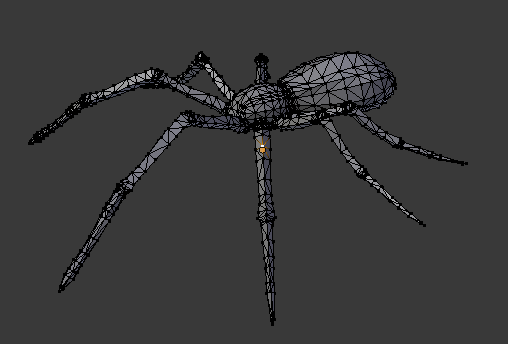
\includegraphics[height=6 cm]{figures/spiderMesh.png}
\caption{A simple spider mesh model. \protect\cite{spiderMesh}}
\label{fig:spiderMesh}
\end{figure}
There are two general methods to manipulate polygon meshes of articulated creature such as the spider. The first approach is to use a pure scene graph approach. But there are three main problems: first problem is how to represent a node in a scene graph. In the previous simple robot example, since the components of robot are all primitive graphics such as sphere and cylinder, the axis could be considered as an abstraction to represent a node. However for a more complex polygon meshes model such as spider shown in figure \ref{fig:spiderMesh}, since the edges of components are irregular, it is hard to find some abstraction layer to represent a node. The other two problems are vertices are changing in local coordinate system and hard to estimate the real outcome of the animation. As a result the project will adopt skeletal modeling, rigging and skinning should be done. 
Most modeling software such as 3DMax, Blender has the function of automatic rigging. However, it is most for human figures. So in this stage, the rigging and skinning of the spider will be done manually by using Blender. An example of spider rigging done manually by using Blender can be seen in figure \ref{fig:spiderRigging}.
 \begin{figure}[ht!]
\centering
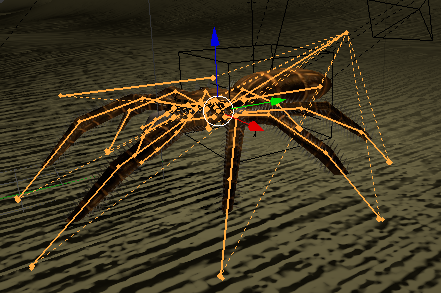
\includegraphics[height=6 cm]{figures/spiderRigging.png}
\caption{A rigging spider example. \protect\cite{spiderModel}}
\label{fig:spiderRigging}
\end{figure}
Also in this stage, a configuration file about biological modeling which mainly covers the limitations of a real creature such as DOF of all joints and speed limitations will be made. The data will be adopted from biology or observations of the natural extent of the spider posture.
\section{Spider animation}
The realism of the spider animation depends on two aspects: First, it should have some different behavior patterns to show its intelligence. Here behavior patterns could be wander, seek food, jump. Secondly, the details of how it take a step.
The three layers of locomotions from \cite{steering} provides a main scheme for this project. The three layers of locomotion is action selection, steering behavior and locomotion behavior. \cite{thesis} implemented the arthropod simulation also on the schema but used a hybrid approach of procedural and physically based animation. The steering behavior in \cite{thesis} acts as a middle layer of delivering forces according what the action selection is and also maintain the overall kinematics of the spider. The difference between \cite{thesis} and this project is instead of considering how the forces are delivered, the project will considering maintain relation table which deals with the relations between the action selection and rules will applied to the spider. Here rules mainly deals with the kinematics. In sum, the three layers design provides the solution of how to show the intelligence of the spider and a scheme of the animation part of the project.
Since the first layer which is the action selection layer is intended to solve the problem of intelligence of the spider. There are two subtasks in it. The first is to define a table which maintains the relation between action selection and pace. A normal spider pace pattern description could be seen in \cite{arsimu2}. A similar pattern which is usually used as normal hexapod gait is shown in figure \ref{fig:triGait}.
 \begin{figure}[ht!]
\centering
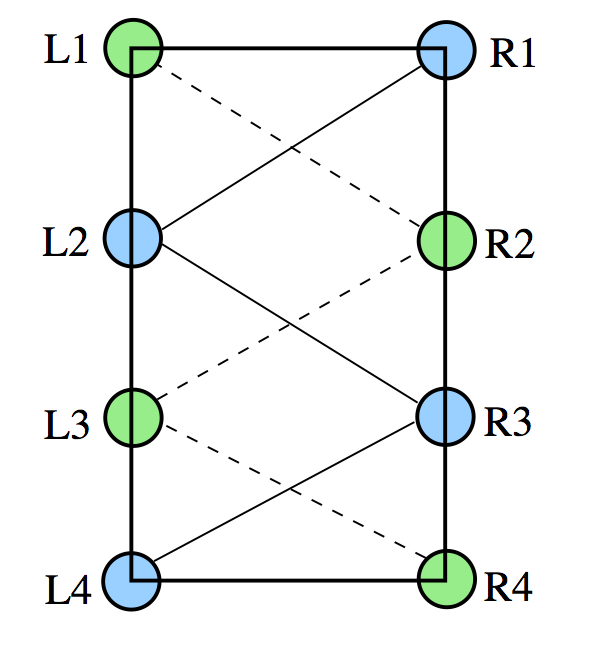
\includegraphics[height=6 cm]{figures/triGait.png}
\caption{The Tripod Gait. \protect\cite{thesis}}
\label{fig:triGait}
\end{figure}
A simple implementation of using the tripod gait shown in \ref{fig:triGait} could be lifting up the limbs in the same color at the same time. Limbs in different color are stepping in turns. However in reality, usually the limbs in the same color are not exactly at the same time. For example, when the limb L1 lift up a bit, then the limb R2 begun lifting. So the timing of how each limb lift up is very important. Figure \ref{fig:gaitTiming} is the timing strategy adopted by \cite{thesis}. The limbs in the different color are corresponding to the gait pattern in figure \ref{fig:triGait}.
 \begin{figure}[ht!]
\centering
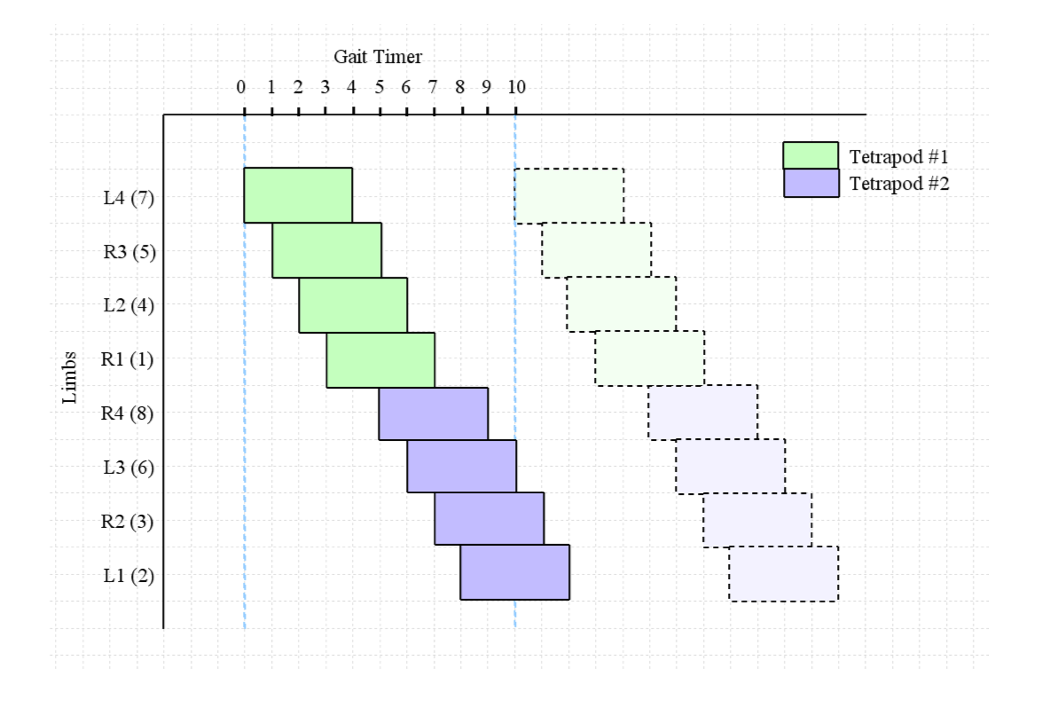
\includegraphics[height=6 cm]{figures/timing.png}
\caption{The Gait Timing. \protect\cite{thesis}}
\label{fig:gaitTiming}
\end{figure}
But the pattern of the steps will not fit with the behavior such as explore or wander. When the spider explore, the spider may use the front limbs to detect the front places to check whether the terrain is uneven or is there a wall before it. The gait pattern may be keep waving the two front limbs, other limbs are moving backward and forwards a bit. While when the spider wander, the heading may change frequently, so one side of the limbs may step more frequently than the other side. The seeking food behavior may be dependent the extent of hunger of the spider, if the spider is a little hunger, it may step more frequent. But when it suddenly find a food near it, it may just directly jump. And if the spider is very hungry, it may not have strength, so it will step very slowly and even without lifting some limbs. The picture could be like a spider use some of its legs to drag the whole body. But due to the fact that it is very hard to estimate the difficulty of implementation. The project first will add the basic behavior such as simple walk, jump and climb walls. If time allowed, behaviors mentioned above will be added to the project. 
A sense module also need to be built because a sense module could solve some action such as seek food or walk on a ball surface\cite{thesis}. It should have two parts which are the foot detection and the ability to see. The second layer is the steering layer which mainly deals with the velocity of the spider according to which action is selected. Though forces will not be considered in the project, acceleration is still needed to be considered. The basics of implementation may be similar to the game SuperMario mentioned in chapter 2. The difference is the acceleration will not triggered by the player but by the coeffect of the environment and the current behavior pattern.  
The last part is to solve how the steering behavior could fit with the pace pattern proposed above. The major part of this stage is mainly to use inverse kinematics with the pattern of the steps. Two approaches which could solve the inverse kinematics are Cyclic Coordinate Descent and Jacobian Transpose.
\section{Spider rendering}
As stated before, the main task of spider rendering is mostly to render the details of the spider. There are three main approaches to render fur which are polygon strip approach, texels approach and shells approach\cite{fur}. The polygon strip approach is easier than the other two approaches. The texels approach is the one which could best results but resource demanding. The shells approach take the concept of the texels approach but implemented the same idea with traditional texture mapping approaches\cite{fur}. The first and third approach are two most popular approaches to render the fur of the spider. Apart from the fur, there are also other aspects could be considered such as using bump mapping to show indents or using soft shadows to make the spider more real. But as stated before, the project will use a very basic rendering which maybe just setting the material property without using texture at all. If time allowed, techniques mentioned in this chapter will be considered.
\section{Oculus Rift}
The Oculus Rift is a virtual reality headset developed by Oculus VR. It enables users to seamlessly look around the virtual world. It tracked every little movement of users' head to create a natural experience. Further more, it provides a stretching world view instead the traditional way which limited users' eyes in a boxed screen.\cite{rift1}
It publishes its SDK which could be integrated ether into OpenGL or Unity3D. Due to the easy setup of Oculus Rift with Unity3D by plugins, the project will choose Unity3D as the main developing software.
\section{Requirements Lists}
\begin{itemize}
  \item \textbf{Extensibility}  
The project should provide a configuration file which could be easily altered by non-programmers to change the details of spider animation which include the basics of animation such as the DOF of the joint between the abdomen and thorax, the max speed of the spider and the details of the intelligent behavior which may be the scope of area of the eyes of the spider.
 \item \textbf{Basic Animation} 
  The spider should have abilities to walk on flat surface and a sphere surface. The spider should have basic behaviors: climb walls and jump. If no advanced behavior is triggered and there is no any user input, the spider will fall into default mode in which a spider will explore the areas in these basic animations.
\item \textbf{Advanced behaviors}
  The spider should have at least one advanced behavior mentioned in section 3.3 such as seek food. When the advanced behavior is triggered, the way the spider moves such as the stepping pattern and speed will change accordingly; for example, if the user throw a piece of food within the spider's view, the spider will jump or run to the food. However, the advanced behaviors will be determined by the progress of the project which means the final advanced behavior may not contain the seek food but will contain at least one mentioned in section 3.3.
 \item \textbf{User Control}
 In order to observe the animation conveniently, user interface will be implemented to handle following functions:
 \begin{itemize}
  \item ability to zoom or change the position and orientation of the camera.
  \item ability to trigger the advanced behaviors of the spider
  \item ability to control the spider(e.g. move and jump)
 \end{itemize}
\end{itemize}
\section{Testing and Evaluation}
\subsection{Testing}
It is hard to predict the final results and approaches adopted in the final project for lack of experience in relevant projects. The main development method adopted is agile software development. Prototype of the project meeting part of requirements will be implemented very quick. As a result, the testing phase will be embedded in different phase of the development and black-box testing will be used. 
In black-box testing, the expected output is the actual image of the spider of animation of the spider. The input are methods adopted or parameters which affect the animation. Since there may be lots of changes in the project, testing will be mainly integration and system testing. 
\subsection{Evaluation}
\begin{itemize}
  \item \textbf{Extensibility}  
   The extensibility mainly focus on the configuration file. The ease of use and how many parameters that can be altered to change the animation could be evaluated. The ease of use means the file should be well organized and has no ambiguities. The parameters could be DOF of each joint, speed, the view scope of the spiders, etc.
  \item \textbf{Realism} 
Two main approaches are proposed to judge the realism of the animation. One is to judge the realism by users based on their memories of spider movement. The other is to compare the animation with real video.
\item \textbf{Rendering}
Though the rendering is not required in the project, if rendering techniques other than the smooth rendering adopted, it should be considered as a bonus to the project. 
\end{itemize}
\section{Ethics and Legal considerations}
One big problem of using Oculus Rift is causing motion sickness\cite{motionSick}. It is common in first-person shooter video game such as Counter-Strike. So the users should be warned about the motion sickness issues before he wears the Oculus Rift device. Also because by using Oculus Rift, the user is so deeply immersed in the virtual reality that he may not pay attention to real environment. For example, he may want to step back when a spider comes close to him which may cause injury. So a third person should be around the users who use the device. 
There is another issue about the fear of spiders. A banner or sign should be placed in obvious places to indicate the issues and in the meantime the users should be notified about all the issues above verbally.
According to the guides and code in \cite{ushuman}\cite{ukhuman}\cite{humanPro}, human participants should be informed the risks of the experiment, the values of the experiment and sign a form of written informed consent or parental permission. However due to the fact that most cases involving human participants are usually medical or psychological and the project does not have the same extent level of risks. For the project, all the risks mentioned above along with the usage of project should be stated clear in a print form documentation, and need users to sign the form before use the Oculus Rift device.
